\newcommand{\layerheight}{2};
\newcommand{\neuronwidth}{1.5};
\newcommand{\neuron}[3]{\draw[fill, white] (#1 * \neuronwidth, #2 * \layerheight) circle (0.5); \draw (#1 * \neuronwidth, #2 * \layerheight) circle (0.5) node {#3};}
\newcommand{\neuronconn}[4]{\draw (#1 * \neuronwidth, #2 * \layerheight) -- (#3 * \neuronwidth, #4 * \layerheight);}
\newcommand{\neuronconnst}[5]{\draw[#5] (#1 * \neuronwidth, #2 * \layerheight) -- (#3 * \neuronwidth, #4 * \layerheight);}

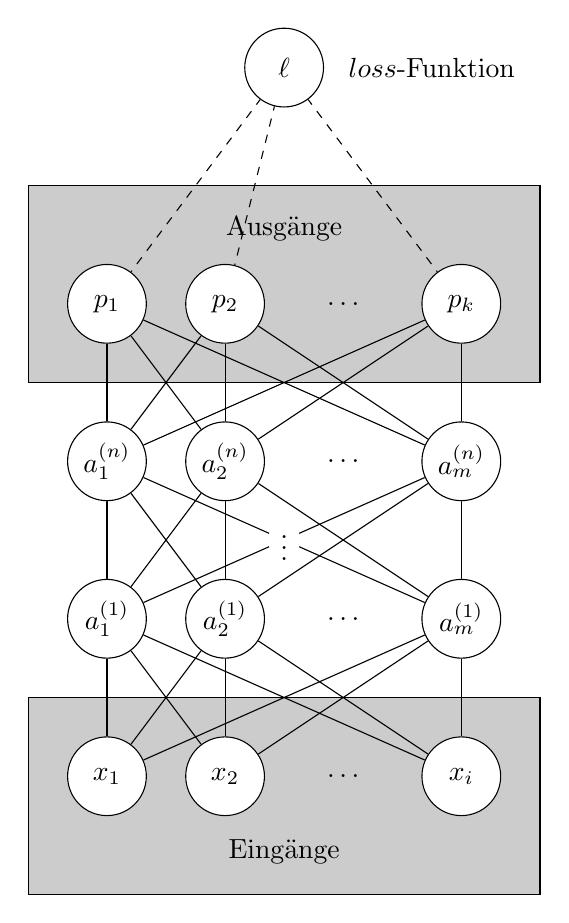
\begin{tikzpicture}
	\draw[fill=black!20] (-1, -1.5) rectangle (5.5, 1) node[midway, yshift=-20] {Eingänge};
	\draw[fill=black!20] (-1, 5 / 2 * \layerheight) rectangle (5.5, 7.5 / 2 * \layerheight) node[midway, yshift=20] {Ausgänge};

	% Verbindungen
	\neuronconn{0}{0}{0}{1}
	\neuronconn{0}{0}{1}{1}
	\neuronconn{0}{0}{3}{1}
	\neuronconn{1}{0}{0}{1}
	\neuronconn{1}{0}{1}{1}
	\neuronconn{1}{0}{3}{1}
	\neuronconn{3}{0}{0}{1}
	\neuronconn{3}{0}{1}{1}
	\neuronconn{3}{0}{3}{1}
	
	\neuronconn{0}{1}{0}{2}
	\neuronconn{0}{1}{1}{2}
	\neuronconn{0}{1}{3}{2}
	\neuronconn{1}{1}{0}{2}
	\neuronconn{1}{1}{1}{2}
	\neuronconn{1}{1}{3}{2}
	\neuronconn{3}{1}{0}{2}
	\neuronconn{3}{1}{1}{2}
	\neuronconn{3}{1}{3}{2}
	
	\neuronconn{0}{2}{0}{3}
	\neuronconn{0}{2}{1}{3}
	\neuronconn{0}{2}{3}{3}
	\neuronconn{1}{2}{0}{3}
	\neuronconn{1}{2}{1}{3}
	\neuronconn{1}{2}{3}{3}
	\neuronconn{3}{2}{0}{3}
	\neuronconn{3}{2}{1}{3}
	\neuronconn{3}{2}{3}{3}
	
	\neuronconnst{0}{3}{1.5}{4.5}{dashed}
	\neuronconnst{1}{3}{1.5}{4.5}{dashed}
	\neuronconnst{3}{3}{1.5}{4.5}{dashed}
	
	% Eingänge
	\neuron{0}{0}{$x_1$}
	\neuron{1}{0}{$x_2$}
	\draw (2 * \neuronwidth, 0 * \layerheight) node {$\dots$};
	\neuron{3}{0}{$x_i$}
	
	% 1. Layer
	\neuron{0}{1}{$a_1^{(1)}$}
	\neuron{1}{1}{$a_2^{(1)}$}
	\draw (2 * \neuronwidth, 1 * \layerheight) node {$\dots$};
	\neuron{3}{1}{$a_m^{(1)}$}
	
	\draw[fill, white] (3 / 2 * \neuronwidth, 1.5 * \layerheight) circle (0.2);
	\draw (3 / 2 * \neuronwidth, 1.5 * \layerheight) node {$\vdots$};
	
	% n. Layer
	\neuron{0}{2}{$a_1^{(n)}$}
	\neuron{1}{2}{$a_2^{(n)}$}
	\draw (2 * \neuronwidth, 2 * \layerheight) node {$\dots$};
	\neuron{3}{2}{$a_m^{(n)}$}
	
	% Ausgänge
	\neuron{0}{3}{$p_1$}
	\neuron{1}{3}{$p_2$}
	\draw (2 * \neuronwidth, 3 * \layerheight) node {$\dots$};
	\neuron{3}{3}{$p_k$}
	
	% Training
	\neuron{1.5}{4.5}{$\ell$}
	\draw (1.5 * \neuronwidth +1.25 * \neuronwidth, 4.5 * \layerheight) node {$loss$-Funktion};
\end{tikzpicture}